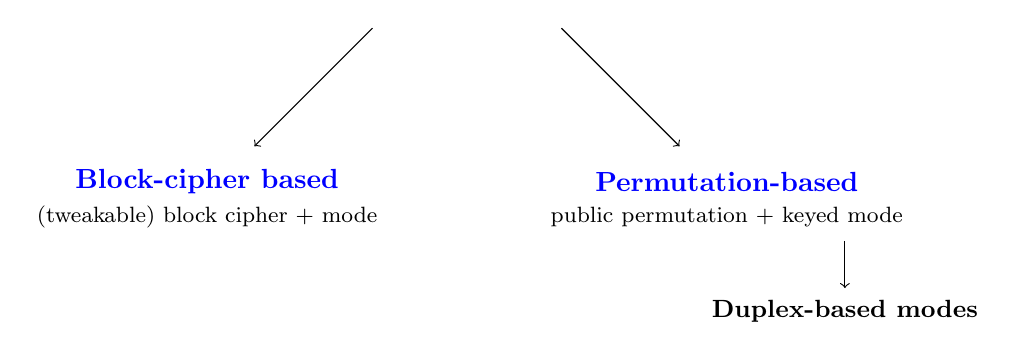
\begin{tikzpicture}[scale=0.3]

\tikzset{SpongePerm/.style=rounded corners=4pt,};
%\tikzset{edge/.style=-latex new, arrow head=8pt};
%\tikzset{edgee/.style=latex new-latex new, arrow head=8pt};



\begin{scope}


\draw[->] (-4,0) -- ++(-5,-5);
\draw(-11,-6.5) node{\color{blue}\textbf{Block-cipher based}};
\draw(-11,-8) node{\footnotesize (tweakable) block cipher + mode};

\draw[->] (4,0) -- ++(5,-5);
\draw(11,-6.5) node{\color{blue}\textbf{Permutation-based}};
\draw(11,-8) node{\footnotesize public permutation + keyed mode};

\draw[->] (16,-9) -- ++(0,-2);
%\draw(10,-14) rectangle ++(12,3);
\draw(16,-12) node{\small \textbf{Duplex-based modes}};


\end{scope}

\end{tikzpicture}
